



\documentclass[10pt]{article}



\usepackage{graphicx, amssymb, latexsym, amsfonts, amsmath, lscape, amscd,
amsthm, color, epsfig, mathrsfs, tikz, enumerate}


\setlength{\topmargin}{-1.5cm}
\setlength{\textheight}{23cm} \setlength{\textwidth}{16cm}    \setlength{\oddsidemargin}{0cm} \setlength{\evensidemargin}{0cm} 




\vfuzz2pt \hfuzz2pt \newtheorem{theorem}{Theorem}[section]
\newtheorem{conjecture}[theorem]{Conjecture}
\newtheorem{corollary}[theorem]{Corollary}
\newtheorem{example}[theorem]{Example}
\newtheorem{lemma}[theorem]{Lemma}
\newtheorem{proposition}[theorem]{Proposition}
\newtheorem{question}[theorem]{Question}
\newtheorem{problem}[theorem]{Problem}
\newtheorem{observation}[theorem]{Observation}
\newtheorem{defn}[theorem]{Definition}
\newtheorem{rem}[theorem]{Remark}
\newtheorem{claim}{Claim}

\newcommand\DELETE[1]{}
\newcommand\ES[1]{\textcolor{red}{#1}}
\newcommand\ESOK[1]{#1}



\begin{document}

\title{{\bf On homomorphism of oriented graphs with respect to push operation}}
\author{ {\sc Sagnik Sen}\\
\mbox{}\\
{\small Indian Statistical Institute, Kolkata, India}
}


\date{\today}

\maketitle

\begin{abstract}
An oriented graph is a directed graph without any cycle of length at most 2. 
 To push a vertex of a directed graph is to reverse the orientation of the arcs incident to that vertex.
Klostermeyer and MacGillivray  defined push graphs which are equivalence class of oriented graphs with respect to vertex pushing operation. 
They studied the homomorphism of the equivalence classes of oriented graphs with respect to push operation.  
In this article, we further study the same topic and answer some of the questions asked in the above mentioned work. 
The anti-twinned  graph of an oriented graph is obtained by adding and pushing a copy of each of its vertices. 
In particular, we show that two oriented graphs are in a push relation if and only if they have isomorphic anti-twinned graphs. 
Moreover, we study oriented homomorphisms of outerplanar graphs with girth at least five, planar graphs and planar graphs with girth at least eight with respect to the push operation.  
\end{abstract}

\noindent \textbf{Keywords:} oriented graphs, push operation, graph homomorphism, chromatic number, planar graphs.



\section{Introduction and preliminaries}


An {\textit{oriented graph}} 
 is a directed graph with no cycle of length 1 or 2. By replacing each edge of a simple graph  with an arc (ordered pair of vertices)
  we obtain an oriented graph ;   is  an \textit{orientation} of  and  is the \textit{underlying graph} of .
  We denote by   and )   respectively  the set of vertices  and arcs  of .   
For an arc  the vertex  is an \textit{in-neighbor} of  and  is an \textit{out-neighbor} of . 
 The set of all in-neighbors and the set of all out-neighbors of  are denoted by  
  and , respectively. 



Let  and  be two oriented graphs. 
A homomorphism of  to  is a
 mapping  which preserves the arcs, that is,  implies . 
 We write  whenever there exists a 
 homomorphism of  to  and say that  \textit{bounds} .   
 The \textit{oriented chromatic number}  of an oriented graph  is 
 then the minimum order  of an oriented graph  such that

admits a homomorphism to ~\cite{orientedchi}.





  To \textit{push} a vertex  of a directed graph  is to change the 
  orientations  of all the arcs (that is, to replace the arc  by ) incident with . 
  Vertex pushing  of directed graphs has been studied by several 
  researchers~\cite{fisher-push, klostermeyer1, klostermeyer2, Mosesian, Pretzel1, Pretzel2, Pretzel3, Garyandwood}
  while Ochem and Pinlou~\cite{OPgirth4} used 
the push operation on oriented graphs for 
proving  the 
upper bounds of the  oriented chromatic number for  the families of triangle-free planar graphs and of 2-outerplanar graphs. 
Finally, Klostermeyer and MacGillivray brought these two popular field of studies 
together in their work~\cite{push} and considered the push operation on oriented graphs to define  equivalence classes of oriented graphs and studied homomorphisms between them. 

  
  

  Two  oriented graphs 
 and  are in a \textit{push relation} if it is possible to obtain  by pushing some vertices 
 of .
 Note that this push relation is in fact an
equivalence relation. A \textit{push graph}   is an equivalance class of oriented
graphs 
(where  is an element of the equivalence class) with respect to the
above mentioned relation. 
An element   of the equivalence class  is a
\textit{presentation} of . 
We use the notation   
for
  is a
presentation of .  
  
 

Note that the graphs having a push relation have the same underlying graph. Hence, we can define the \textit{underlying graph} of a push graph  by the underlying graph of any presentation of it and 
denote it by . 
The \textit{order} of a push graph is the number of vertices of its underlying graph, hence can be denoted by 
 or . 
Intuitively, we can treat a push graph as an oriented graph whose arcs, incedent to a vertex, are able to switch directions. 
Given  any oriented graph  we can consider the corresponding push graph 
. 


A push graph  admits a homomorphism  to an oriented graph 
 if there exist  a presentation 
 such that  is a homomorphism of   to 
. We write  whenever there exists a 
 homomorphism of  to .

A push graph  admits a homomorphism  to a push graph 
 if there exist presentations 
 and 
   
such that  is a homomorphism of   to 
. 
 We write  whenever there exists a 
 homomorphism of  to  and say that  \textit{bounds} . 
      As in  general graph homomorphisms, for push graphs also, a bijective homomorphism whose inverse is also a 
     homomorphism is 
     an \textit{isomorphism}. 


The push chromatic number  of the push graph  is the minimum order  of a push graph  such that

admits a homomorphism to .  
It is equivalent to say that the push chromatic number  of the push graph  is the minimum order  of an oriented graph  such that

admits a homomorphism to .  




The push chromatic number  of  an undirected graph 
  is the maximum of the push chromatic numbers of all the push graphs with underlying graph  . The push chromatic number  of  a family  of graphs is the maximum of the push  chromatic numbers of the graphs from the family .


\begin{figure}


\centering
\begin{tikzpicture}


\filldraw [black] (.5,1.5) circle (2pt) {node[below]{}};
\filldraw [black] (.5,2.5) circle (2pt) {node[above]{}};


\filldraw [black] (3.5,1.5) circle (2pt) {node[below]{}};
\filldraw [black] (3.5,2.5) circle (2pt) {node[above]{}};


\draw[->] (.5,1.5) -- (.5,2);
\draw[-] (.5,2) -- (.5,2.5);


\draw[->] (3.5,1.5) -- (3.5,2);
\draw[-] (3.5,2) -- (3.5,2.5);

\draw[-<] (.5,1.5) -- (2.5,2.16);
\draw[-] (2.5,2.16) -- (3.5,2.5);






\draw[-<] (3.5,1.5) -- (1.5,2.16);
\draw[-] (1.5,2.16) -- (0.5,2.5);



\draw[thick] (.5,2) ellipse (0.6cm and 1.1cm);
\draw[thick] (3.5,2) ellipse (0.6cm and 1.1cm);

\node at (-1,2) {};

\node at (.5,3.8) {};

\node at (.5,3.4) {};


\node at (.5,3.4) {};


\node at (2,0) {\textbf{(a)}};




\filldraw [black] (7,1.5) circle (2pt) {node[below]{}};
\filldraw [black] (9,1.5) circle (2pt) {node[above]{}};


\filldraw [black] (7,3.5) circle (2pt) {node[below]{}};
\filldraw [black] (9,3.5) circle (2pt) {node[above]{}};


\draw[-<] (7,1.5) -- (8,1.5);
\draw[-] (8,1.5) -- (9,1.5);


\draw[-<] (7,3.5) -- (8,3.5);
\draw[-] (8,3.5) -- (9,3.5);

\draw[-<] (7,1.5) -- (7,2.5);
\draw[-] (7,2.5) -- (7,3.5);

\draw[->] (9,1.5) -- (9,2.5);
\draw[-] (9,2.5) -- (9,3.5);


\node at (8,0) {\textbf{(b)}};


\end{tikzpicture}

\caption{\textbf{(a)} The anti-twinned graph  of . \textbf{(b)} A push invarient graph .}\label{fig anti-twinned graph orientable}

\end{figure}


Klosetermeyer and MacGillivray~\cite{push} showed that deciding whether a push graph admits a -push coloring or not is 
 NP-complete   for .  
In their paper, they  suggested several future directions regarding the topic among which we address here the following ones:

\begin{itemize}
\item[\textbf{(A)}] Is it true that two oriented graphs belong to  the same equivalence class  if and only if their anti-twinned (defined in Section~\ref{sec results}) graphs are isomorphic
 (see Fig.~\ref{fig anti-twinned graph orientable}(a))?


\item[\textbf{(B)}] What are the outerplanar graphs that have push chromatic number three.

\item[\textbf{(C)}] Investigating push chromatic  number for different graph families, especially, families of planar graphs.
\end{itemize}



In Section~\ref{sec results}  we address the above three points. First we will show that the question asked in \textbf{(A)} has a positive answer.  
Then we prove that outerplanar with \textit{girth} (length of the smallest cycle) at least five admits a push 3-coloring 
while observing that it is not possible to relax the girth restriction from that result. This will partially answer point \textbf{(B)}.
Then we deal with point \textbf{(C)} and  show that the push chromatic number of planar graphs lies between 10 and 40. 
Moreover, we prove that the push chromatic number for the family of planar graphs with girth 8 is 4.
 




 
 
 
 
 

 
 



\section{Results}\label{sec results}
The anti-twinned graph  of an oriented graph 
  
  was defined and used by Klostermeyer and MacGillivray in~\cite{push}.

Let  be a push graph with vertex set  and 
. Then the
\textit{anti-twinned graph}  of  is the oriented graph with the set of vertices and the set of arcs as the following (also see Fig.~\ref{fig anti-twinned graph orientable}(a)):
 
 
 
 


 
 
 
  Intuitively,  is the graph obtained from  by adding and pushing  a twin vertex   for each of the vertices  of . 
  Observe that  is well defined upto isomorphism, that is, for any presentation of 
  , we will get the same oriented graph . 
  

Now we will prove a result which answers point \textbf{(A)}
mentioned in the introduction.

 
 \begin{theorem}\label{corollary push and oriented}
Two oriented graphs  and   are in the same  equivalence class with respect to the push operation if and only if 
their corresponding anti-twinned graphs  and  are isomorphic.
 \end{theorem}
 
 
 \begin{proof}If  and   are in the same push equivalence class then 
 their corresponding anti-twinned graphs  and  are isomorphic was shown by Klostermeyer and MacGillivray~\cite{push}. So it is enough to prove only the ``if'' part of the theorem.
 
 
For any isomorphism  of  to  define the set 
 
Furthermore,  if  is a vertex of an oriented graph  then  denotes its corresponding anti-twin in . Moreover, we fix the convention .
 
 
 
 Let  and  be two oriented graphs and let  be an isomorphism of 
  to . Note that if  then we are done. 
 
 
 
 Therefore, let , that is,  . Now we define the following: 




Intuitively, we just interchanged the images of  and  to obtain . As  was a bijective function from  to , so is . 
If we can show that both  and  are oriented graph homomorphisms between  and , then we will 
end up proving that  is an oriented graph isomorphism of 
  to . For convenience let . 


First we will show  that  is a homomorphism of  to . Let  be an arc in 
. If  then there is an arc from  to  as  itself  
is an isomorphism. 

Now suppose  and . This implies . Therefore, 

Similarly, one can argue for the case when  and .

Then suppose that  and . 
This implies . 
Hence  
Similarly, one can argue for the case when  and .

Note that  and  are non-adjacent. Hence,  and  are also non-adjacent. Therefore,  and 
are non-adjacent. That takes care of the case when .

\medskip

Now we will prove that  is a homomorphism. 
Let  be an arc in 
.
If  then there is an arc from  to  as  itself  
is an isomorphism. 


Now suppose  and . 
This implies  
Therefore, 


Similarly, one can argue for the case when  and .

Then suppose that  and . 
This implies  
Hence 

Similarly, one can argue for the case when  and . 

\medskip

So we have shown that  is an isomorphism. Also note that ,  and either 
or . 
Hence . 

So we can recursively define a chain of isomorphisms 
 of  to   so that we have 

This completes the proof.
 \end{proof}

\bigskip


Now we will prove a result that will give us more insight regarding the relation between oriented graph homomorphism and push operation and also help us to prove a particular step of an upcoming theorem. 


\begin{proposition}\label{th any target}
Let  be a homomorphism of  to . 
Then for each presentation  there exists a presentation 
 such that  is a homomorphism of 
to .
\end{proposition}

\begin{proof}
Let  be a homomorphism of  to  and  
be any presentation.  Suppose one can obtain  from  by pushing the set of vertices 
. Now obtain the presentation  from  by 
pushing the pre-images of , that is, the set of vertices . It is easy to check that 
 is a homomorphism of 
to .
\end{proof}

















 


A \textit{splitable oriented graph}  is an oriented graph isomorphic  to the anti-twinned graph   of some oriented graph . The oriented graph  is the \textit{split graph} of .
The following two results will be instrumental in proving other results of this article.


\begin{observation}\label{push why splitable}
An oriented graph  is splitable if and only if it is possible to partition the set of vertices   into two equal parts  and  with a bijection  such that 
 for all  we have  and . 
\end{observation}

The above result follows directly from the definition of splitable oriented graph. 

\begin{lemma}\label{lem split implies good}
Let  be a splitable graph. Then  
if and only if . 
\end{lemma}


\begin{proof}
Let  be a splitable graph. 
Assume that . This implies 
. 
Now consider the following function  from  to :



It is easy to check that  is a homomorphism of 
 to . This implies that there exists a 
push homomorphism . By composing this 
homomorphism with the homomorphism 
we obtain a homomorphism . 
This proofs the ``only if'' part.

For proving the  ``if'' part assume . Then 
we have  due to Klostermeyer and MacGillivray~\cite{push}. 
By composing this homomorphism with the inclusion homomorphism of 
 to  we will be done.
\end{proof}



An outerplanar graph is a graph that can be drawn on a plane with all its vertices lying on a circle and all its edges can be drawn inside the circle without any crossing. Klostermeyer and MacGillivray~\cite{push} showed that the family of outerplanar graphs has 
push chromatic number 4. 


\begin{theorem}\mbox{}\label{pushouter}
Let  be the family of outerplanar graph with girth at least five. Then  .
\end{theorem}

\begin{proof}
In~\cite{outergirth}, Pinlou and Sopena showed that every outerplanar graph with girth at least 
and minimum degree at least 2 contains a face of length  with at least  consecutive vertices of degree 2.
We will show that every push outerplanar graph of girth at least 5 admits a homomorphism to the directed 3-cycle . 


Let  be a minimal (with respect to inclusion as a
subgraph) push outerplanar graph with girth at least 5 having no homomorphism to .

\begin{itemize}

\item[(i)]  Suppose that  contains a vertex  of degree 1. Then, due  to the minimality of 
, 
the push outerplanar graph obtained by deleting the vertex  from  (which has girth at least 5) admits a homomorphism to . 
Since every vertex of  has in-degree and out-degree equal to 1, the homomorphism can easily be extended to obtain a homomorphism of  to  , 
a contradiction.

\item[(ii)] Suppose that  contains a face  of length  with at least  consecutive vertices  of degree 2. Then, due  to the minimality of 
, 
the push outerplanar graph  obtained by deleting the vertices 
 from  (which has girth at least 5) admits a homomorphism  to . 
 Now, let  be a presentation of  with 
 . Note that 
 the vertices  and  are adjacent in . 
 Hence, . 

It is possible to check that (a bit tidious, but not difficult, by case analysis), given any oriented path of length , with edges  and a mapping 
 with , it is possible to push the vertices  for  to obtain an oriented path and extend the mapping  to a homomorphism of that oriented path to .

Hence, by the above observation, we can extend the homomorphism of  to  to a homomorphism of  to , 
a contradiction.

As any  cycle of odd length has push chromatic number at least 3, the  bound is tight. 
\end{itemize}
\end{proof}


\medskip

An undirected simple  graph  admits an \textit{acyclic -coloring} if it can be colored by  colors 
in such a way that the graph induced by each color is an independent set and the graph induced by a pair of colors is a forest. 
This definition was introduced in~\cite{acyclic-def}.

\begin{theorem}\label{pushacyclic}
Every graph with acyclic chromatic number at most  has push chromatic number at most . 
\end{theorem}


\begin{proof}
For any positive integer  the \textit{Zielonka graph}~\cite{orientedchi}   of order  is  the oriented graph with    set of vertices   where 




\noindent and  set of arcs  


 
\medskip 
 
Furthermore, note that the vertices of a   can be partitioned into two disjoint sets of equal size





Also, we can define a function  by  where the  operation is taken modulo 2. It is clear that  is a bijection of the type described in Observation~\ref{push why splitable}. 
Hence  is 
a splitable oriented graph. 
Therefore, . 


Now let  be a push graph and its underlying simple graph  admits an acyclic -coloring. 
Raspaud and Sopena~\cite{planar80} showed that the oriented graph  admits an oriented homomorphism to . 
Hence by Lemma~\ref{lem split implies good}  where  
is the oriented graph induced from  by . 
Clearly,  is a graph on 
 vertices, hence we are done. 
\end{proof}

As 
~\cite{push}, 
the upper bound of the above result is tight for  due to Ochem~\cite{Ochem_negativeresults}.
Now we establish the lower and upper bounds for the push chromatic number of  planar graphs.



\begin{theorem}\label{th p3}
Let  be the family of all planar graphs. Then . 
\end{theorem}



\begin{proof}
Borodin~\cite{Borodinacyclic} 
showed that every planar graph 
admits an acyclic 5-coloring. 
Hence the upper bound follows by Theorem~\ref{pushacyclic}.


\medskip

Now we will prove the lower bound. 

\medskip


\textbf{\textit{Claim 1:}} There exists an oriented graph  on  vertices such that every
planar push graph admit a homomorphism to . 

\medskip

\textit{Proof of the claim:} Let  be the set of all oriented graphs of order  
. If our claim is false then for each  there exists a planar push graph 
 that does not admit a homomorphism to . 
Let  be the disjoint union of all such graphs. Note that  is a planar graph and does not admit homomorphism to any oriented graph on  vertices and thus have , a contradiction. \hfill 

\medskip



We say an oriented graph  has property \textbf{(P1)} if  is an oriented graph on 
   vertices such that every
planar push graph admits an homomorphism to . 
Moreover,   is minimal such graph with respect to subgraph inclusion. 

By the above claim we are garunteed that there exists an oriented graph  with property \textbf{(P1)}.
First note that if  has \textbf{(P1)} then by Proposition~\ref{th any target} any presentation of  also have  property \textbf{(P1)}.
Note that the graph obtained by reversing all the arcs of  any graph with  property \textbf{(P1)} also has property \textbf{(P1)}. 

Two vertices  and  of an oriented graph agree on a third vertex  if  for 
some . Similarly, 
 and  disagree on   if  for . Let  denote the set of vertices that  and  agree on and let  denote the set of vertices that  and  disagree on. Note that 
given two vertices  and  of a fixed oriented graph the sets  and  remains as it is under push operation unless you push exactly one of . If you push exactly one of  then the two sets get interchanged. 
Therefore, the parameters  and  are push invarient. 



Let  be an arc of . Then push all in-neighbors of . Now if in the so-obtained presentation  we have , then stop. 
Otherwise, 
push the vertex  and reverse all the arcs of  and stop. Call the graph obtained in the final step 
. Notice that,    has property \textbf{(P1)}. Moreover, all neighbors of  in 
 are out-neighbors and we have .


\medskip

\textbf{\textit{Claim 2:}} If two vertices  and   of a push graph has  then they cannot have the same image under any homomorphism. 


\medskip

\textit{Proof of the claim:} Let the 4-cycle drawn in Fig~\ref{fig anti-twinned graph orientable}(b) be the graph . Note that this graph is push invarient and 
no two of its vertices can  have the same homomorphic image.
Also any two vertices of a push graph with  must be part of a subgraph isomorphic to .
\hfill 

\medskip

 
























 \medskip




\begin{figure} 


\centering
\begin{tikzpicture}





\filldraw [black] (8,0) circle (2pt) {node[below]{}};
\filldraw [black] (10,0) circle (2pt) {node[below]{}};
\filldraw [black] (12,0) circle (2pt) {node[below]{}};

\filldraw [black] (10,2) circle (2pt) {node[right]{}};

\filldraw [black] (8,4) circle (2pt) {node[above]{}};
\filldraw [black] (10,4) circle (2pt) {node[above]{}};
\filldraw [black] (12,4) circle (2pt) {node[above]{}};

\filldraw [black] (6,2) circle (2pt) {node[left]{}};








\draw[->] (8,4) -- (9,3);
\draw[-] (9,3) -- (10,2);


\draw[->] (10,4) -- (10,3);
\draw[-] (10,3) -- (10,2);


\draw[->] (12,4) -- (11,3);
\draw[-] (11,3) -- (10,2);

\draw[->] (10,2) -- (9,1);
\draw[-] (9,1) -- (8,0);

\draw[->] (10,2) -- (10,1);
\draw[-] (10,1) -- (10,0);



\draw[->] (10,2) -- (11,1);
\draw[-] (11,1) -- (12,0);

\draw[->] (8,0) -- (9,0);
\draw[-] (9,0) -- (10,0);

\draw[->] (10,0) -- (11,0);
\draw[-] (11,0) -- (12,0);

\draw[->] (8,4) -- (9,4);
\draw[-] (9,4) -- (10,4);

\draw[->] (10,4) -- (11,4);
\draw[-] (11,4) -- (12,4);



\draw (10,0) .. controls (9,-2) and (8,-2) .. (6,2);

\draw[->] (8.8,-1.3) -- (8.8001,-1.3);




\draw (10,4) .. controls (9,6) and (8,6) .. (6,2);

\draw[->] (8.8,5.3) -- (8.8001,5.3);




\draw (12,0) .. controls (10,-4) and (8,-4) .. (6,2);

\draw[->] (9.3,-2.8) -- (9.3001,-2.8);


\draw (12,4) .. controls (10,8) and (8,8) .. (6,2);

\draw[->] (9.3,6.8) -- (9.3001,6.8);






\draw[->] (6,2) -- (7,1);
\draw[-] (7,1) -- (8,0);

\draw[->] (6,2) -- (8,2);
\draw[-] (8,2) -- (10,2);

\draw[->] (6,2) -- (7,3);
\draw[-] (7,3) -- (8,4);







\end{tikzpicture}

\caption{A planar graph  of order 8 with .}\label{fig push planarmax}
\end{figure}


Due to the minimality of  there exists a planar push graph  with the following property: 
if  is a homomorphism of a presentation  to   then 
 for each arc  there exists an arc 
 such that  and . 




Now we construct an oriented planar graph  by gluing a copy of the planar graph  (Fig.~\ref{fig push planarmax})
to each vertex of  by identifying the vertex with the vertex  of .
Then we glue the gadget graph   (Fig.~\ref{fig gadget})
to each vertex of  by identifying the vertex with the vertex  of  and obtain a new oriented graph .
Note that the gadget graph  is planar and thus   is also planar. 
After that we construct another oriented planar graph  by gluing a copy of the planar graph  
to each arc of  by identifying the arc with the arc  of .


Note that each pair of  non-adjacent vertices of the oriented planar graph  from Fig~\ref{fig push planarmax}
is part of a common . 
So no two vertices of  can have the same homomorphic image 
and thus . 
Moreover,  in  . Also as no two vertices of  can be identified,
if  admits a homomorphism  to a graph  then   in 
. 

Consider the push graph  of the gadget graph  (Fig.~\ref{fig gadget}). Here  the vertices  and  must have different image under any homomorphism as any pair of them are part an . Also the vertices of the directed 5-cycle that is induced by the common neighbors of  and  must have distinct images under any homomorphism. Hence 
if  admits a homomorphism  to a graph  then   in 
. Similarly, we will have   in .




 Therefore,  each vertex in  has degree at least 7 and for each arc  of  we have . Also for each vertex  of  there are at least two vertices  and  of 
  with .



Theerefore,  for each vertex  of   there exists a 
 vertex  of 
with  and . That is,   and  have at least 7 common neighbors. Thus  has at least 
9 vertices and if  has exactly 9 vertices  then it is a tournament.

\medskip







\begin{figure} 


\centering
\begin{tikzpicture}



\filldraw [black] (-4,2) circle (4pt) {node[above]{}};

\node at (-4,2.35) {\textbf{\textit{v}}};

\draw[->][very thick] (-3.5,2) -- (-1,2);




\filldraw [black] (0,0) circle (2pt) {node[below]{}};
\filldraw [black] (2,0) circle (2pt) {node[below]{}};
\filldraw [black] (4,0) circle (2pt) {node[below]{}};


\filldraw [black] (0,4) circle (2pt) {node[below]{}};
\filldraw [black] (2,4) circle (2pt) {node[below]{}};
\filldraw [black] (4,4) circle (2pt) {node[below]{}};

\filldraw [black] (0,2) circle (2pt) {node[below]{}};
\filldraw [black] (4,2) circle (2pt) {node[below]{}};


\filldraw [black] (2,1) circle (3pt) {node[above]{}};
\filldraw [black] (2,3) circle (3pt) {node[below]{}};

\draw[->] (2,1) -- (1,.5);
\draw[-] (1,.5) -- (0,0);

\draw[->] (2,1) -- (2,.5);
\draw[-] (2,.5) -- (2,0);

\draw[->] (2,1) -- (3,.5);
\draw[-] (3,.5) -- (4,0);

\draw[->] (2,1) -- (1,1.5);
\draw[-] (1,1.5) -- (0,2);

\draw[-<] (2,1) -- (3,1.5);
\draw[-] (3,1.5) -- (4,2);



\draw[->] (2,3) -- (1,2.5);
\draw[-] (1,2.5) -- (0,2);

\draw[->] (2,3) -- (2,3.5);
\draw[-] (2,3.5) -- (2,4);

\draw[->] (2,3) -- (3,2.5);
\draw[-] (3,2.5) -- (4,2);

\draw[->] (2,3) -- (1,3.5);
\draw[-] (1,3.5) -- (0,4);

\draw[-<] (2,3) -- (3,3.5);
\draw[-] (3,3.5) -- (4,4);





\draw[->] (0,0) -- (1,0);
\draw[->] (1,0) -- (3,0);
\draw[-] (3,0) -- (4,0);

\draw[->] (4,0) -- (4,1);
\draw[-] (4,1) -- (4,2);


\draw[->] (4,2) -- (2,2);
\draw[-] (2,2) -- (0,2);

\draw[->] (0,2) -- (0,1);
\draw[-] (0,1) -- (0,0);


\draw[->] (0,2) -- (0,3);
\draw[-] (0,3) -- (0,4);



\draw[->] (0,4) -- (1,4);
\draw[->] (1,4) -- (3,4);
\draw[-] (3,4) -- (4,4);

\draw[->] (4,4) -- (4,3);
\draw[-] (4,3) -- (4,2);








\end{tikzpicture}

\caption{The gadget graph . The thick arrow suggests that there are arcs from  to every other vertices except  and .}\label{fig gadget}
\end{figure}



 
 



Now for the rest of the proof we will assume that  is a tournament on 9 vertices and prove the theorem by contradicting 
this assumption.
 
 
First recall that there is a vertex  of  such that . Moreover, there is a vertex  of  such that . This implies  and .
Now suppose that  and . 


For any  vertex  we have . 
Thus we must have  for all .


\medskip

\textbf{\textit{Claim 3:}} Each vertex  must have exactly 1 in-neighbors in . 

\medskip

\textit{Proof of the claim:} Suppose a vertex  does not have exactly 1 in-neighbors in . Then one of the following cases hold:

\begin{itemize}
\item[]  Suppose  has no in-neighbors in . That means . As  , there can be  at most 1 out-neighbor of  in . The set  contains the vertex , out-neighbors of  in  and in-neighbors of  in . Thus , a contradiction. 

\item[]  Suppose  has exactly 2 in-neighbors in .  As  , there must be at  least 2 out-neighbor of  in . 
Thus there is at most 1 in-neighbor of  in . The set  contains in-neighbors of  in  and out-neighbors of  in . 
Thus , a contradiction. 


\item[]  Suppose  has exactly 3 in-neighbors in .  As  , there must be at  least 3 out-neighbor of  in . 
Thus there is no in-neighbor of  in . The set  contains in-neighbors of  in  and out-neighbors of  in . 
Thus , a contradiction. \hfill 
\end{itemize}

 
\medskip



As  and , by pigeonhole principal, there are two vertices  with a common in-neighbor in .
That implies the other two vertices of  are common out-neighbors of  and . Thus . 
Therefore, . That implies , a contradiction.
\end{proof}
















Note that, improving the upper bound will improve the long standing 
upper bound of oriented chromatic number of planar graphs. Indeed our result uses the proof of  the later. 
Whereas our lower bound proof is independent of the lower bound proof for oriented chromatic number of planar graphs by Marshall~\cite{marshall18}. 
Moreover, a lower bound of 9 for the push chromatic number of planar graphs can be achieved using Marshall's result 
while we provide a better lower bound of 10 for the same. Even though our lower bound does not imply any improvement of Marshall's lower bound of 18
for oriented chromatic number of planar graphs, it does imply the following corollary.

\begin{corollary}\label{cor 19?}
There exists no splitable oriented graph on 18 vertices to which every oriented planar graph admits a homomorphism to. 
\end{corollary}

A graph is called a \textit{core graph} if it does not admit a homomorphism to any of its proper subgraph~\cite{hell}.  The unique~\cite{hell} subgraph to which 
a graph admits a homomorphism to is called its \textit{core}. 
Marshall~\cite{marshall17} first established the lower bound of 17 for oriented chromatic number of planar graphs by showing that there exists no oriented graph on 16 vertices to which every planar graph admits a homomorphism to. 
For proving this first he showed that the Tromp graph~\cite{marshall17}  on 16 vertices is the only graph to which every planar graph can admit a homomorphism to. Then he constructed an example of an oriented planar graph that does not admit a homomorphism to .
After that Marshall~\cite{marshall18} extended his result to prove that the only oriented graph on 17 vertices to which all planar graphs can admit a homomorphism to is an oriented graph whose core is . 
An easy but significant observation is that the family of Tromp graphs, in particular , are splitable graphs. 
So if one can show that the only possible oriented core graph on 18 vertices to which every planar graph admits a homomorphism to is a splitable graph, then by our result the lower bound for oriented chromatic number can be improved to 19.

\medskip

\noindent \textbf{Question:} Is it possible to get rid of the word ``splitable'' from Corollary~\ref{cor 19?}?

\medskip
   
Now we will prove a tight bound for push chromatic number for the family of planar graphs with girth at least 8.



















\begin{theorem}\label{th p8}
Let  be the family of all planar graphs with girth at least 8. Then . 
\end{theorem}

\begin{proof}
If , then we can prove that there exists a tournament on 3 vertices to which every 
planar push graph with girth at least 8 admits a homomorphism to by mimiking the proof of claim~1 of Theorem~\ref{th p3}. 
Now, upto push euivalence, there is only one tournament, the directed 3-cycle ,  on three vertices. 
Therefore, given any planar graph  with girth at least 8, there   must be a presentation 
of   that admits a homomorphism to the directed 3-cycle  by Proposition~\ref{th any target}. 

Take the directed    9-cycle . Now construct the graph  by taking 
   and a new vertex  and then connecting each vertex of  to  by two distinct paths of length 4 (one of them directed and the other with three forward arcs and one backward arc). 
Now consider the push graph . 

Notice that for any presentation  we will have  one 4-path, 
with either three forward arcs and one backward arc or with three backward arcs and one forward arc, connecting  to each vertex of the 9-cycle. 

Observe  that the 4-path  with three forward arcs and one backward arc 
does not admit a homomorphism with  and  mapped to the same vertex of .
Now let  be a homomorphism of  to . Then, because of the above observation, 
 for every vertex  from the 9-cycle. But we know that the 9-cycle has push chromatic 
number equal to 3. That means  must be onto on the vertices of  when restricted to 
the 9-cycle. Hence . This is a contradiction.
Hence we have the lower bound.  

\medskip


For proving the upper bound it is enough to show that every push  with  
maximum average degree less than    admits a homomorphism to the Paley plus graph  due to Borodin,  Kostochka, 
 Ne\v{s}et\v{r}il,  Raspaud and Sopena~\cite{mad}. 
We will use the discharging method for our proof. 


We first provide a (small) set of \textit{forbidden confgurations}, that
is a set of graphs that a minimal counterexample  to our claim cannot contain
as subgraphs. We will then assume that every vertex  in  is valued by its degree
 and define a \textit{discharging procedure} which specifies some transfer of values
among the vertices in , keeping the sum of all the values constant. We will then get
a contradiction by considering the \textit{modernized degree}  of every vertex , that
is the value obtained by  owing to the discharging procedure.


\medskip


\textbf{\textit{Drawing conventions:}} In all the figures depicting forbidden configurations, we will
draw vertices with prescribed degrees as `square vertices' and vertices with unbounded
degree as `circular vertices'. All the neighbors of square vertices are drawn. Unless otherwise
specified, two or more circular vertices may coincide in a single vertex, provided
that they do not share a common square neighbor. 




\textbf{\textit{Observation 1:}} It is easy to check that 

and   for all . 



First assume that  is a mimimal (with respect to the number of vertices) push graph
with maximum average degree less than  that does not admit a homomorphism to
 . 



\begin{figure} 


\centering
\begin{tikzpicture}


\filldraw [black] (-4,5) circle (2pt) {node[below]{}};
\filldraw [black] (-3,6) circle (2pt) {node[below]{}};
\filldraw [black] (-2,5) circle (2pt) {node[below]{}};
\filldraw [black] (-3,7) circle (2pt) {node[below]{}};


\draw[->] (-4,5) -- (-3,5);
\draw[-] (-3,5) -- (-2,5);



\draw[->] (-2,5) -- (-2.5,5.5);
\draw[-] (-2.5,5.5) -- (-3,6);


\draw[->] (-3,6) -- (-3.5,5.5);
\draw[-] (-3.5,5.5) -- (-4,5);


\draw[->] (-3,7) -- (-2.5,6);
\draw[-] (-2.5,6) -- (-2,5);


\draw[->] (-3,7) -- (-3,6.5);
\draw[-] (-3,6.5) -- (-3,6);


\draw[->] (-3,7) -- (-3.5,6);
\draw[-] (-3.5,6) -- (-4,5);


\node at (-3,4) {};



\path (0,6) edge (1,6);


\filldraw [black] (0,6) circle (2pt) {node[below]{}};

\filldraw [black] ([xshift=-2pt,yshift=-2pt]1,6) rectangle ++(4pt,4pt) {node[above]{}};


\node at (.5,5) {};


\filldraw [black] (2,6) circle (2pt) {node[below]{}};
\filldraw [black] (5,6) circle (2pt) {node[below]{}};

\filldraw [black] ([xshift=-2pt,yshift=-2pt]4,6) rectangle ++(4pt,4pt) {node[above]{}};
\filldraw [black] ([xshift=-2pt,yshift=-2pt]3,6) rectangle ++(4pt,4pt) {node[above]{}};

\draw[-] (2,6) -- (5,6);

\node at (3.5,5) {};


\filldraw [black] (6,7) circle (2pt) {node[above]{}};
\filldraw [black] (6,5) circle (2pt) {node[above]{}};
\filldraw [black] (9,6) circle (2pt) {node[right]{}};

\filldraw [black] ([xshift=-2pt,yshift=-2pt]7,6.5) rectangle ++(4pt,4pt) {node[above]{}};
\filldraw [black] ([xshift=-2pt,yshift=-2pt]7,5.5) rectangle ++(4pt,4pt) {node[above]{}};
\filldraw [black] ([xshift=-2pt,yshift=-2pt]8,6) rectangle ++(4pt,4pt) {node[above]{}};



\draw[-] (8,6) -- (9,6);

\draw[-] (8,6) -- (6,7);

\draw[-] (8,6) -- (6,5);

\node at (7.5,5) {};


\node at (4,4) {};

\end{tikzpicture}

\caption{ The Paley plus graph .  The forbidden configurations for Theorem~\ref{th p8}.}~\label{figure orientable girth8}

\end{figure}	


First we will show that    does not contain any of the configuration depicted in 
Fig.~\ref{figure orientable girth8}.



\begin{itemize}

\item[(i)] Obvious since every vertex of   has degree at least one.

\item[(ii)] Directly follows from Observation~1.



\item[(iii)] Consider the push graph  obtained by deleting all the square vertex of degree 3 from . Therefore, there exists a presentation 
 such that  admits a homomorphism  to .

Now choose a vertex . 
Suppose that . 

Now consider the presentation  that contains  as a subgraph
and is such that  (such a presentation is possible to obtain by 
pushing  if needed). 

Now we can extend  to a homomorphism 
of  of  to   (by pushing the vertices  and  if needed) with  using 
 Observation~1.

\end{itemize}

We now use the following discharging procedure: each vertex of degree at least
3 gives  
to each of its neighbors with degree .

Let us check that the modernized degree  of each vertex  is at least  which
contradicts the assumption . We consider the possible cases for the old
degree  of :

\begin{itemize}

\item[(i)]  : there is no such vertex in  by (i).

\item[(ii)]: by (ii), both its neighbors have degree at least 3. Therefore, it receives 
exactly
, and thus .


\item[(iii)] : by  (iii),  gives away at most . Therefore, we have 
 .


 \item[(iv)] :  it gives away at most . Therefore, we have 
 .

\end{itemize} 
 
 
 Therefore, every vertex of  gets a modernized degree at least . Hence, every push graph with maximum average degree less than  admits a homomorphism to . 

\end{proof}



\bibliographystyle{abbrv}
\bibliography{POreferences}



 
 
\end{document}
